\chapter{Dataset Preparation }
\label{ch:chapter04}
 
%
% Section: 5 - Intro
%
\section{Introduction}
\label{sec:chapter05:intro}
Software is a real world entity and its mentions in a scientific publications usually appear to be a sequence of tokens.  Therefore, automatic classification of software usage purpose can be modelled as a sequence labeling task in which a class label, from a fixed list of class labels, is assigned to each token in a sequence. \\

Extraction of information about a software can be done following various approaches. In the past, rudimentary approaches such as searching for a term in paper, manual content analysis using human readers as well as rule based approaches have been employed \citep{kruger2019literature}.  More recently a deep learning model have also been employed for extraction of  information about software such as mention types, software type, etc. \citep{schindler2022role}. \\

Sequence labelling is a type of pattern recognition problem, one branch of Natural Language processing (NLP). Examples of classical tasks of sequence labelling are part-of-speech (POS) tagging, named entity recognition (NER), and text chunking \citep{akhundov2018sequence, he2020survey}.  \\

Various types of models that implement sequence labeling can be broadly categorized as machine learning or deep learning based approaches \citep{he2020survey}. Machine learning based models are Hidden Markov Models (HMM) \citep{kupiec1992robust}, Maximum Entropy Markov Models (MEMM) \citep{mccallum2000maximum}, and Conditional Random Fields (CRF) \citep{lafferty2001conditional}.  State-of-the-art sequence labeling model is based on Bi-LSTM-CRF a deep learning neural network architecture. \\

This section explores for models that are suitable for sequence labeling task of automatic classification of software usage purposes. 

\section{Machine learning Models}
\label{sec:chapter05:MLModels}

\subsection{Hidden Markov models (HMMs)}
\label{sec:chapter05:MLModels:HMMS}

One of machine learning models that are used for sequence labeling are Hidden Markov Models (HMMs). HMMs are based on Markov processes which describe a sequence of hidden finite states (Yi) in which a given state in a sequence depends only on the state prior it \citep{enwiki:1071684499, enwiki:1068802172}. \\

As the model transitions through hidden states of Yi, it generates an observation Xi which corresponds to a token in a sentence \citep{aggarwal2018machine}.

\begin{figure}[htbp]
	\centering
	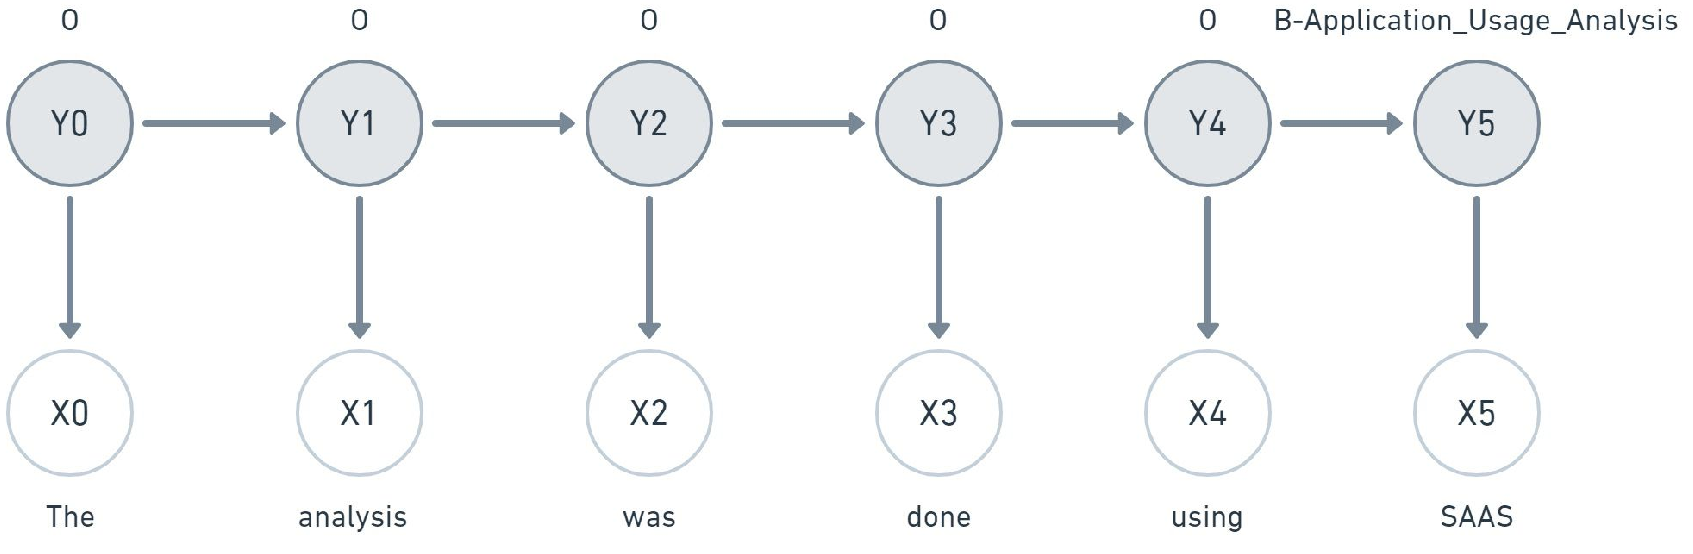
\includegraphics[width=1\textwidth]{4.graphics/figures/models/pdf/HMM}
	\caption{HMM Model}
	\label{fig:chapter03:setup}
\end{figure}

The Markov chain of hidden states generate observations based on its current state using a joint probability distribution p(x,s), hence HMMs are also referred to as generative models. \\

The challenge with Hidden Markov Models is that, it is difficult to define the joint probability because it requires enumeration of all possible observation sequences which makes inference intractable for most applications. In addition, observation sequences in most real-world applications have long-range dependencies and multiple features interacting together \citep{bulla2006application, wallach2004conditional}.
 
\subsection{Maximum Entropy Markov Models (MEMMs)}
\label{sec:chapter05:MLModels:MEMMs}

Unlike hidden Markov models which generate sequences of tokens based on hidden states, maximum entropy models are discriminative models i.e., they model directly model the probability of each label Yi based on the current observation Xi and the prior hidden state Yi-1 \citep{mccallum2000maximum}. 

\begin{figure}[htbp]
	\centering
	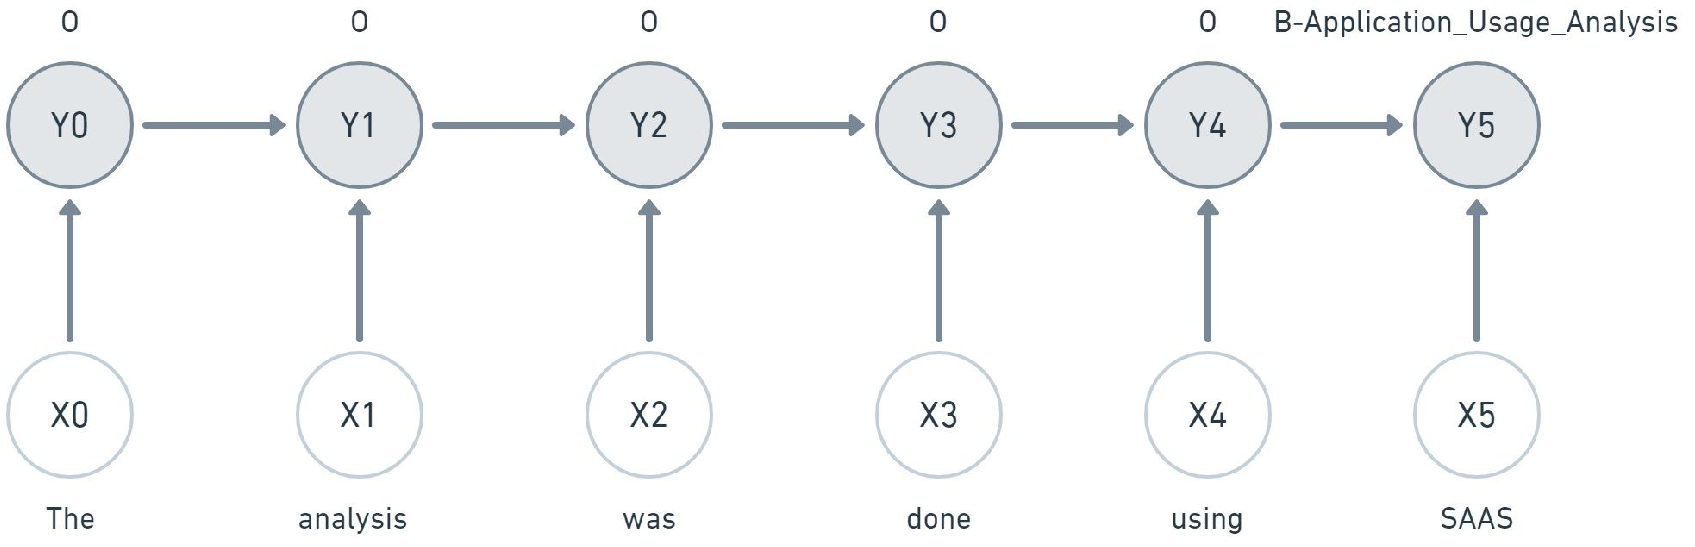
\includegraphics[width=1\textwidth]{4.graphics/figures/models/pdf/MEMM}
	\caption{MEMM Model}
	\label{fig:chapter03:setup}
\end{figure}

The biggest drawback with MEMMs and other discriminative directed graphical models based on Markov, tend to be biased in favor of states with fewer successor states {lafferty2001conditional}. 

\subsection{Linear Conditional Random Fields (CRFs)}
\label{sec:chapter05:MLModels:CRFs}

CRFs are similar with MEMMs in that both are probabilistic and discriminative models that can perform sequence labeling based on conditional probability p(Y|x) unlike joint probability of HMMs \citep{wallach2004conditional}. 

\begin{figure}[htbp]
	\centering
	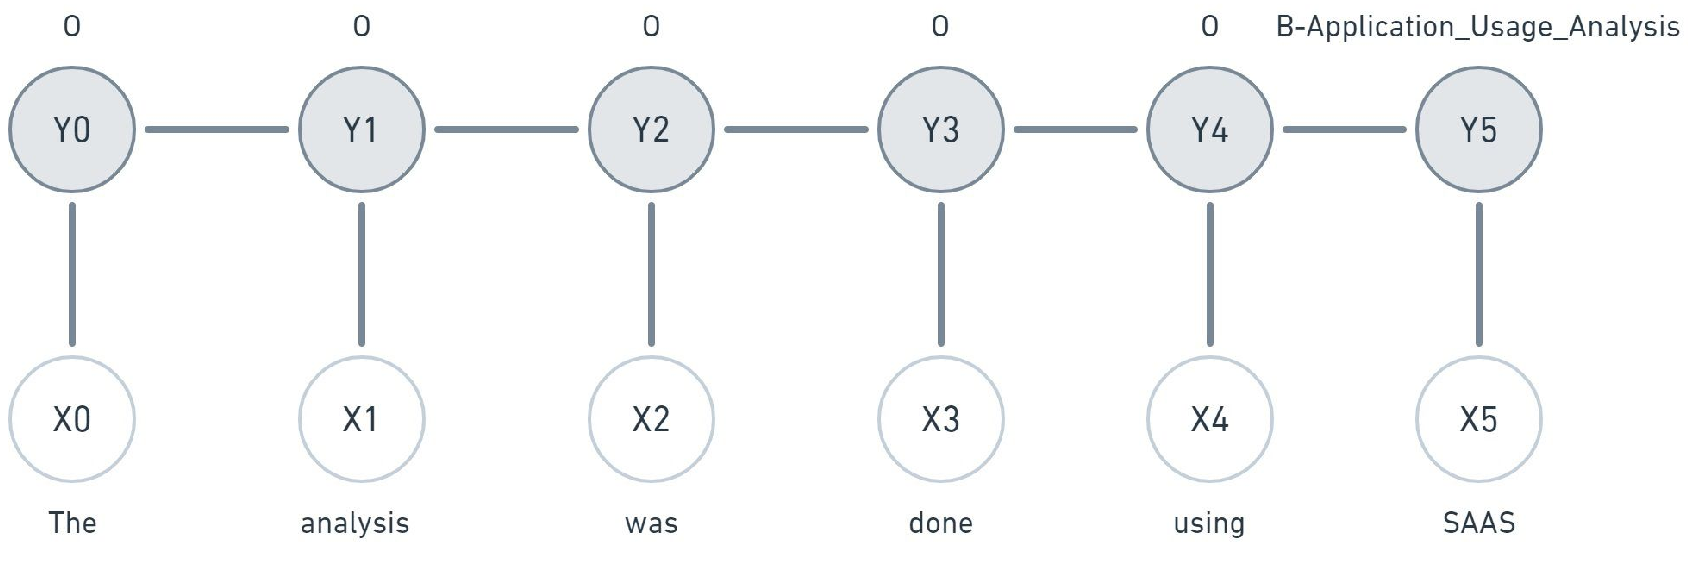
\includegraphics[width=1\textwidth]{4.graphics/figures/models/pdf/CRF}
	\caption{CRF Model}
	\label{fig:chapter03:setup}
\end{figure}

CRFs differ from MEMMs in that they are undirected graphs, i.e., the inference of Yi depends on all the labels occurring before it as well as after it. This makes training of CRFs computationally expensive especially when a wider window of tokens is chosen to handle long range dependencies \citep{aggarwal2018machine}. In addition to inability to capture long-range dependencies, CRFs have another problem, they capture context in a forward direction only \citep{lample2016neural}.



\section{Deep Learning Models }
\label{sec:chapter05:MLModels:DLMs}

Deep learning models yield a state-of-the-art performance for sequence labelling with out the need for manually crafting features because of their ability to automatically learn features from data \citep{he2020survey}. In addition, deep learning models are advantageous because certain variants like LSTMs have the capacity to handle long-term dependencies \citep{akhundov2018sequence}. 



\subsection{Long Short-Term Memory (LSTM)}
\label{sec:chapter05:DLModels:LSTM}

Recurrent Neural Networks (RNNs) are specific type of neural network architectures that take a sequence of inputs Xi and yield another sequence Yi as output. Plain RNNs fail to capture long-range dependencies however a there are other variant of RNNs, such as LSTM networks that are capable of handling long-term dependencies \citep{akhundov2018sequence, lample2016neural}. This is because, unlike conventional feed forward neural networks, LSTMs have feedback mechanism that helps to capture entire sequence of tokens in a sentence enabling the network to remember tokens over arbitrary time intervals \citep{enwiki:1073570927}. 

\begin{figure}[htbp]
	\centering
	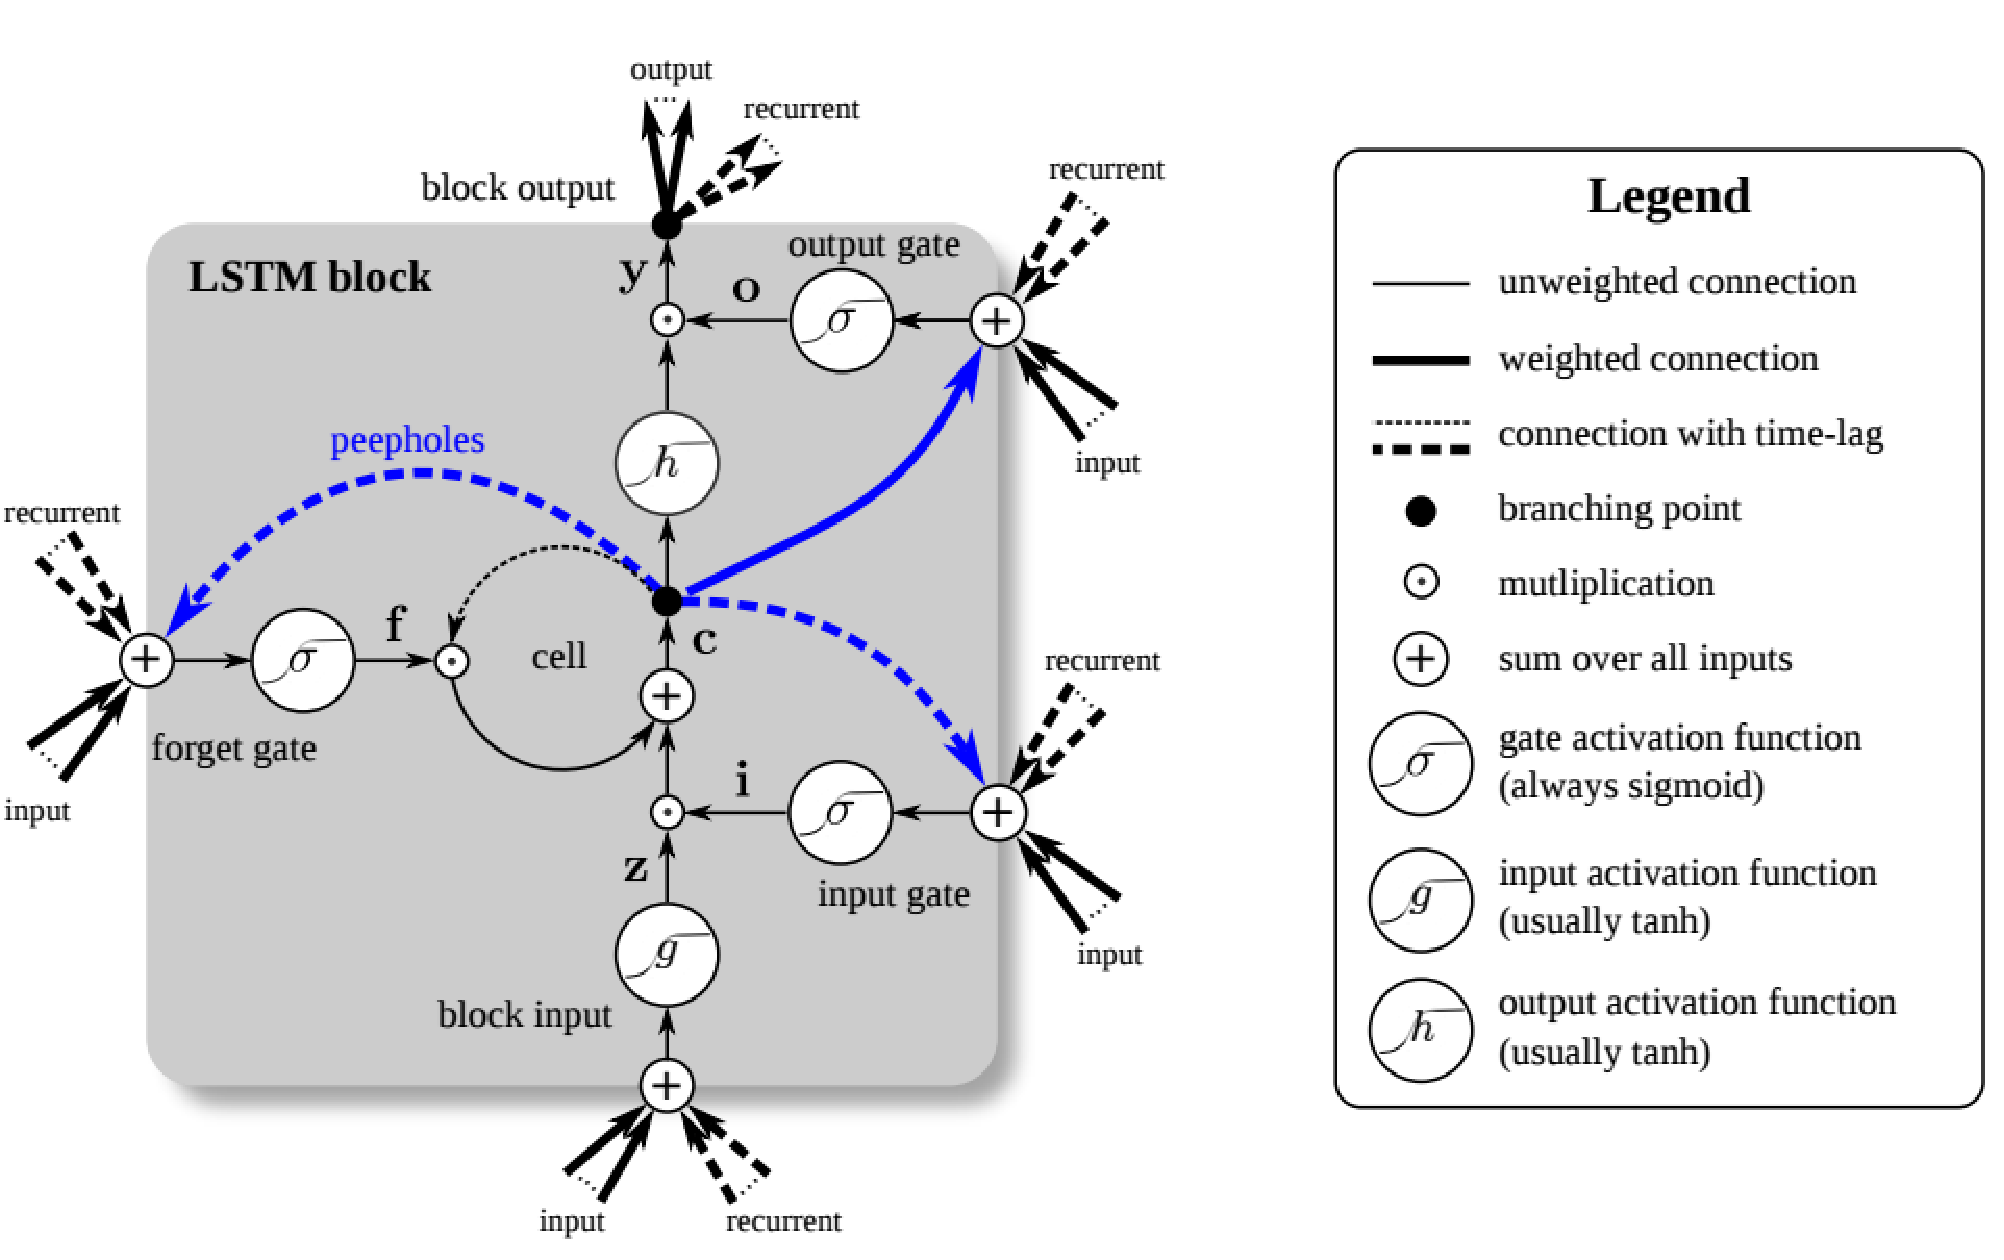
\includegraphics[width=.65\textwidth]{4.graphics/figures/models/pdf/LSTM_cell}
	\caption{LSTM Cell \citep{ma2016end}}
	\label{fig:chapter03:setup}
\end{figure}

A LSTM memory block has three multiplicative components, which determine what amount of information to remember as well as to retain to the next step \citep{ma2016end}. 


\subsection{Bi-Long Short-Term Memory (BLSTM)}
\label{sec:chapter05:DLModels:BiLSTM}

Though LSTM captures the past sequence of tokens (on the left), it is not capable to capture future sequence of tokens. For this reason, two LSTM networks are combined to form Bi-LSTM where one captures context information in a forward direction while the other captures information in the reverse direction. This enables Bi-LSTMs to become aware of both past as well as future contexts \citep{ma2016end}. 

\subsection{Bi-LSTM-CRF}
\label{sec:chapter05:DLModels:BiLSTMCRF}

Bi-LSTM-CRF models are state-of-the-art, elegant solutions to sequence labeling tasks as they are capable of capturing context in both left and right directions due to their Bi-LSTM component. 

\begin{figure}[htbp]
	\centering
	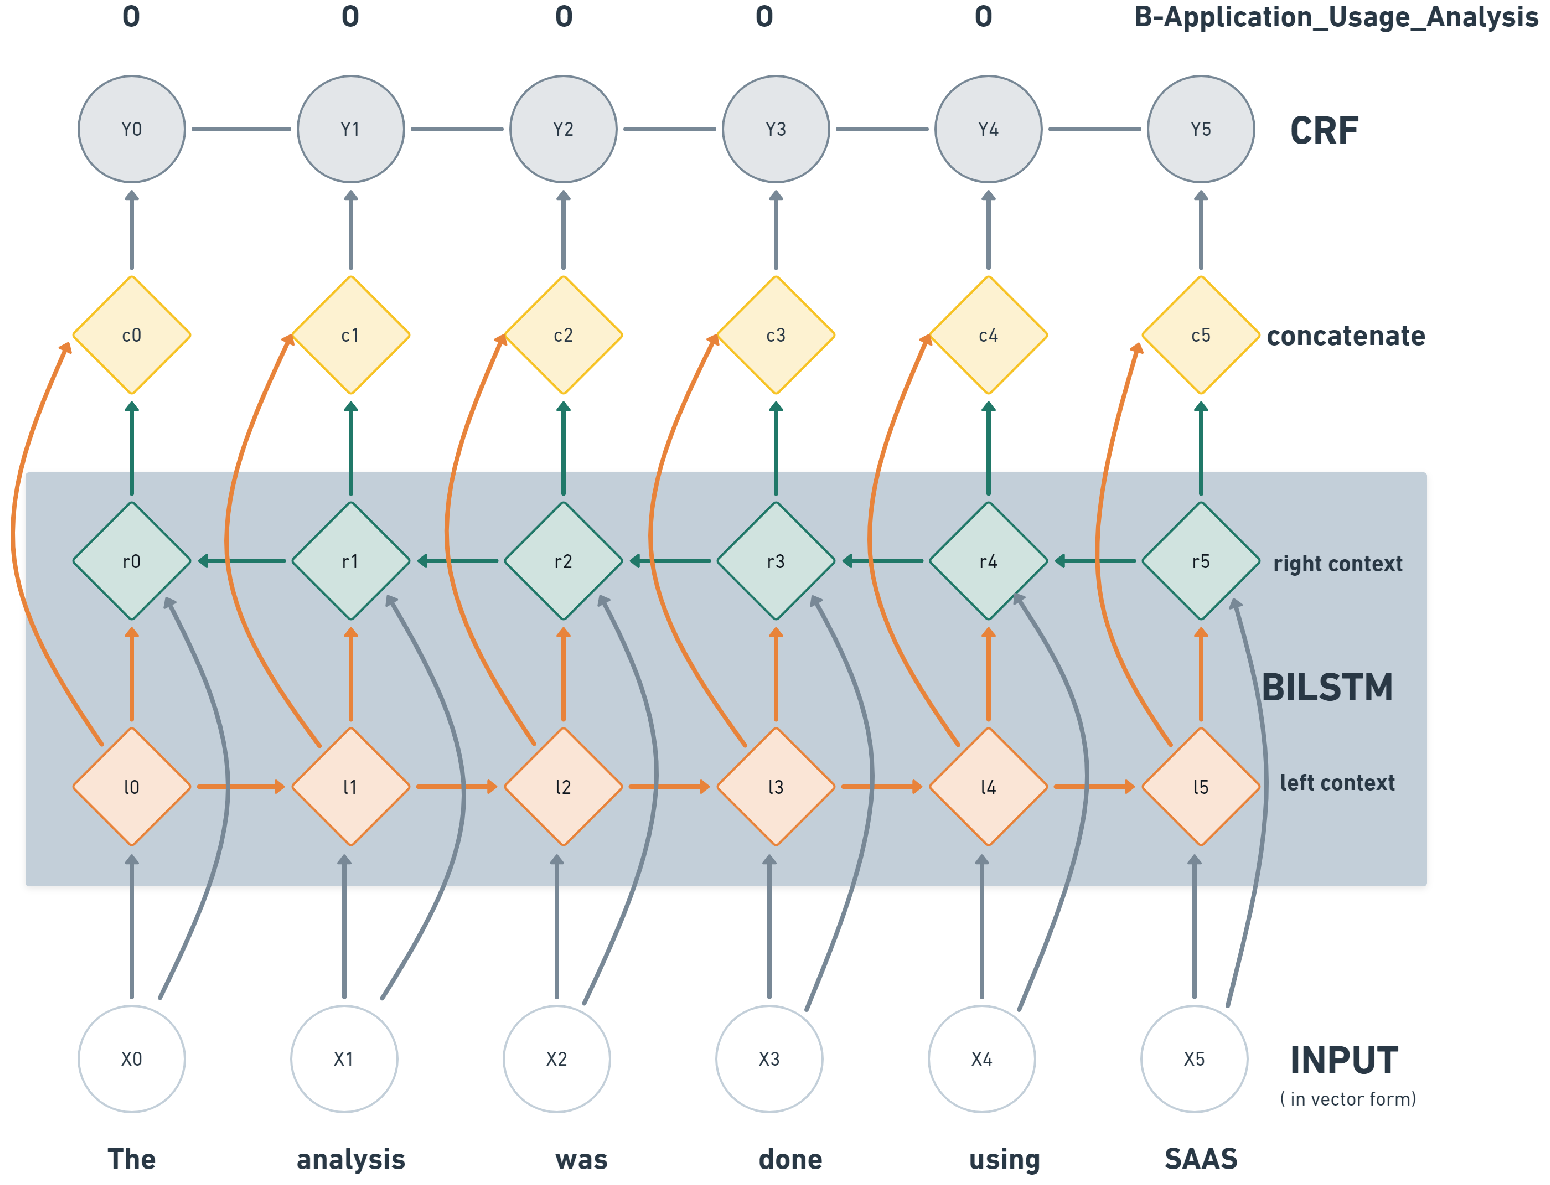
\includegraphics[width=.70\textwidth]{4.graphics/figures/models/pdf/Bi-LSTM-CRF}
	\caption{Bi-LSTM-CRF }
	\label{fig:chapter03:setup}
\end{figure}

Due to its performance Bi-LSTM-CRF model has been employed for classifying software usage purpose from a sequence of tokens in a sentence. The classifier model implemented is a 4 layer network where each classifier layer is dedicated to classifying software, software-type, mention-type and software-purpose in respective order. Fully connected model is shown in the figure below. 

\begin{figure}[htbp]
	\centering
	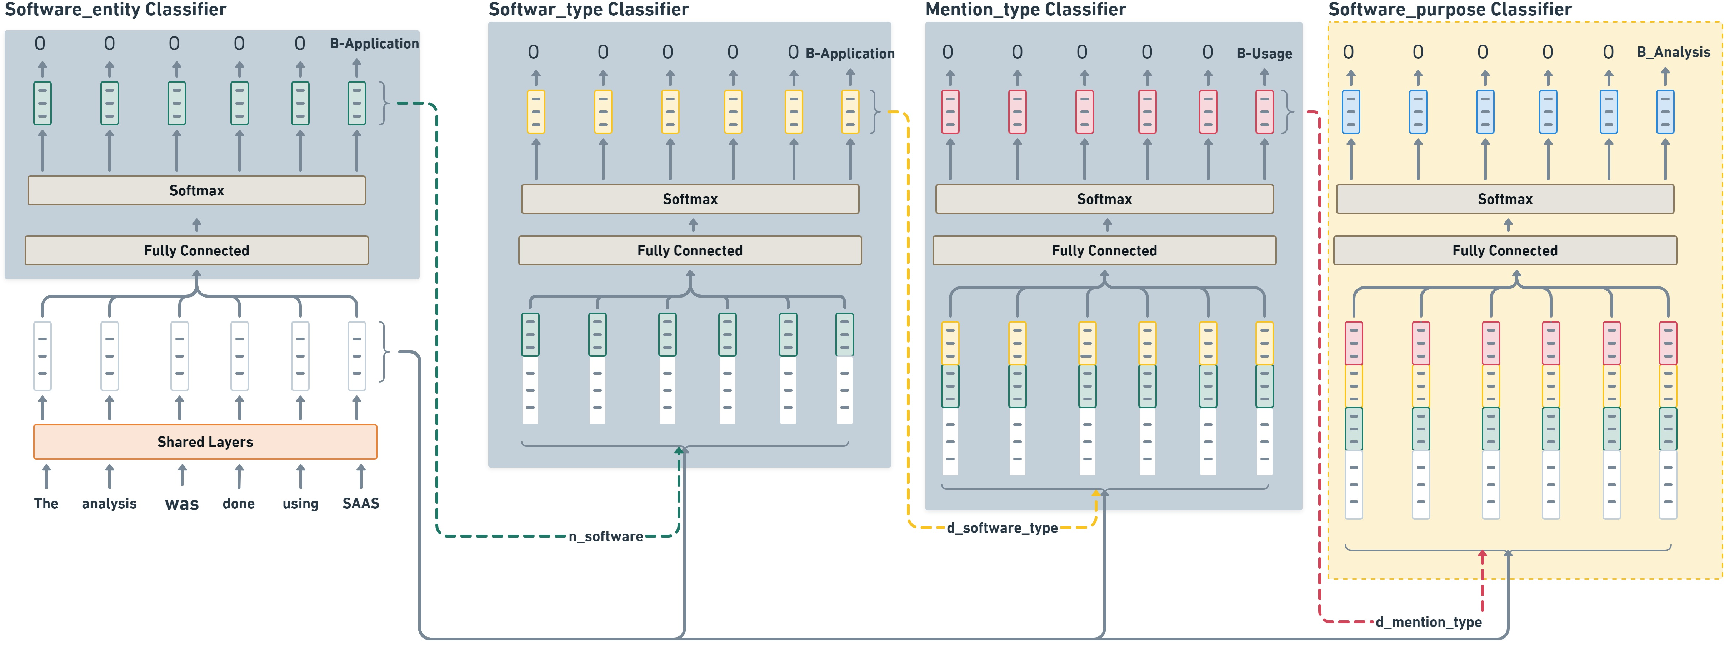
\includegraphics[width=1\textwidth]{4.graphics/figures/models/pdf/fully_connected_model}
	\caption{Fully connected model }
	\label{fig:chapter05:setup}
\end{figure}

\subsection{Word embeddings}
\label{sec:chapter05:DLModels:wemb}

To generate features for each word in a sentence, word embeddings like Sci-BERT and Bio-BERT have been used. Sci-BERT is pre-trained on multi-domain random collection, over 1.14M, of scientific publications and capable of generating contextualized embeddings for each token in a sequence. Most of the scientific papers used to train Sci-BERT are from biomedical domain (82\%) and the rest from computer science domain \citep{beltagy2019scibert}. \\

Bio-BERT is as well a contextualized word embedding trained on biomedical corpora. The scientific publications in the Bio-BERT corpora are made of abstract section of PubMed journal and full text articles from Pub Med Central (PMC) \citep{li2019fine}. 


